%!TEX root = Algebraische_Zahlentheorie.tex

\renewcommand{\lecdate}{21.10.14}
\newpage
\paragraph{Literaturempfehlungen}
\begin{enumerate}[1]
\item BOREVICH, SHAFAREVICH Zahlentheorie
\item CASSELS, FRÖHLICH, Algebraic number theory, Academic Press 1990
\item FRÖHLICH, TAYLOR, Algebraic number theory, CUP 1993
\item LANG, S. Algebraic number theory, Springer 1994
\item MARCUS, D Numberfields, Springer 1995
\item NEUKIRCH, Algebraic number theory, Springer 2002
\item RAMAKRISHNAN, VALENZA, Fourier analysis on numberfields, Springer 1993
\item SWINNERTON-DYER, A brief guide to algebraic number theory, CUP 2001 (nur 147 S.)
\end{enumerate}

\paragraph{Algebraische Voraussetzung}
\begin{itemize}
\item Gruppe, Ring, Körper
\item GALOIS-Theorie
\item Struktursatz über endlich erzeugte Moduln über HIR
\item Elementare Arithmetik: Kongruenzen, $\IF_q\kreuz$ ist zyklisch
\end{itemize}

Siehe z.B. LANG, S.

\newpage
\section{Ganze algebraische Zahlen}
\subsection{Die Mutter aller Ringe: $\IZ$}
$\IZ$ ist kommutativer Ring mit $1$, integer (nullteilerfrei), Quotientenkörper ist $\IQ$.
Wegen des \mbox{EUKLIDischen} Algorithmus ist $\IZ$ ein Hauptidealring, also faktoriell.
Die Einheiten $\IZ\kreuz$ sind $\pm 1$, die Primelemente (= irred. Elemente) sind die Primzahlen und ihre Negativen. Es gibt unendlich viele Primzahlen.
Der klassische Beweis von EUKLID  ist bekannt. Es folgen zwei andere.

\begin{Beweis}[EULER]
Die $n$-te \highl{FERMAT-Zahl} ist
\[F_n=2^{2^n}+1\]
$F_0=3, F_1=5, F_2=17, F_3=257$ und $F_4=65537$ sind Primzahlen. Aber EULER 1732: $F_5=641\cdot 6700417$, denn
$641=5^4+2^4=5\cdot 2^7+1$. Also teilt $641$ die Zahlen $5^4\cdot 2^{28}+2^{32}$ und $5^4\cdot 2^{28}-1$ (dritte binomische Formel) und daher auch die Differenz.

Zeigen nun: Alle zwei verschiedene $F_n$ sind teilerfremd.
Sei $d$ Teiler von $F_n$ und $F_{n+k}$, $k>0$.
\[\frac{F_{n+k}-2}{F_n}=\frac{2^{2^{n+k}}-1}{2^{2^n}+1}=\frac{x^{2^k}-1}{x+1}=x^{2^k-1}-x^{2^k-2}+\ldots-1\in\IN\]
mit $x=2^{2^n}$. Also teilt $F_n$ die Zahl $F_{n+k}-2$, und daher auch $d \mid F_{n+k}-2$. Es folgt $d\mid (F_{n+k}-(F_{n+k}-2))=2$.
Da alle $F_n$ ungerade sind, folgt $d=\pm 1$. Also sind je zwei FERMAT-Zahlen teilerfremd.

Folglich liefert jede FERMAT-Zahl mindestens einen neuen Primfaktor. Also muss es unendlich viele Primzahlen geben.
\end{Beweis}

\begin{Beweis}[EULER]
\[\zeta(s)=\sum_{n=1}^\infty \frac{1}{n^s}\]
bezeichnet die \highl{RIEMANNsche Zetafunktion}. Sie konvergiert für $s>1$. Also $\zeta:(1,\infty)\rightarrow \IR$.
Wir zeigen: $\zeta(s)=\prod_{p\in\IP}\left(1-\frac{1}{p^s}\right)\inv$.
\begin{align*}
\prod_{p\leq x}\left(1-\frac{1}{p^s}\right)\inv&=\prod_{p\leq x} \sum_{m=0}^\infty \frac{1}{p^{ms}}
\end{align*}
Das ist ein endliches Produkt von absolut konvergenten Reihen. Es lässt sich also ausmultiplizieren. Insgesamt erhält man so die Summe aller $\frac{1}{n^s}$, mit $n\in\IN$ und $n=1$ oder alle Primfaktoren $p$ von $n$ erfüllen $p\leq x$. Es folgt daher folgende Abschätzung:
\[0<\zeta(s)-\prod_{p\leq x}\left(1-\frac{1}{p^s}\right)\inv< \sum_{n>x}\frac{1}{n^s}\]
Im Grenzübergang folgt somit die Behauptung:
\[ 0\leq \lim_{x\rightarrow\infty}\zeta(s)-\prod_{p\leq x}\left(1-\frac{1}{p^s}\right)\inv= \zeta(s)-\prod_{p\in\IP}\left(1-\frac{1}{p^s}\right)\inv\leq \lim_{x\rightarrow\infty} \sum_{n>x}\frac{1}{n^s} =0\]
Wegen $\log$ stetig und $\log(1+x)=\sum_{i=0}^\infty(-1)^{i+1}\frac{x^i}{i}$, folgt \[\log{\zeta(s)}=\sum_{p\in\IP}\log\left(\left(1-\frac{1}{p^s}\right)\inv\right)=\sum_{p\in\IP}\log\left(\left(1-\frac{1}{p^s}\right)\inv\right)=\sum_{p\in\IP} \frac{1}{p^s}+ \underbrace{\sum_{p\in\IP}\sum_{n\geq 2} \frac{1}{np^{ns}}}_{(*)}.\] 
Dabei ist $(*)$ für $s\rightarrow 1+0$ beschränkt, denn 
\begin{align*}
\sum_{p\in\IP}\sum_{n\geq 2} \frac{1}{np^{ns}}&<\sum_{p\in\IP}\sum_{n\geq 2} \frac{1}{p^{ns}}=\sum_{p\in\IP}\frac{1}{p^{2s}}\frac{1}{1-\frac{1}{p^s}}\\
&=\sum_{p\in\IP} \frac{1}{p^s(p^s-1)}<\sum_{n=2}^\infty \frac{1}{n^s(n^s-1)}\\
&<\sum_{n\geq 2} \frac{1}{n(n-1)}<\infty
\end{align*}
Also folgt \[\lim_{s\rightarrow 1+0} \sum_{p\in\IP} \frac{1}{p^s}= \sum_{p\in\IP} \frac{1}{p}=\infty.\]
Daher gibt es insbesondere unendlich viele Primzahlen.
\end{Beweis}

\begin{Fakt}[FERMAT]
Eine Primzahl $p$ ist genau dann Summe zweier Quadratzahlen, wenn $p=2$ oder $p\equiv 1 \mod{4}$.
\end{Fakt}

\begin{Beweis}
 Sicher ist $2=1+1$. Für $p\equiv 3 \mod{4}$ hat man keine Chance, denn für alle $n\in\IZ$ ist $n^2\equiv 0$ oder $1 \mod{4}$ ($0$ für $n$ gerade, $1$ für $n$ ungerade). Also ist $m^2+n^2 \equiv 0,1,2 \mod{4}$.
 
Sei nun $p\equiv 1\mod{4}$. $x^2+y^2\equiv 0 \mod{p}$ hat nichttriviale Lösungen genau dann, wenn $-1 =\square$, d.h. $-1$ ist Quadrat, in $\IF_p$. $\IF_p\kreuz$ ist zyklisch \folge $\IF_p\kreuz=\langle g \rangle$. $g^{\frac{p-1}{2}}=-1$. Also $-1=\square$ \gdw $\frac{p-1}{2}$ gerade \gdw $p\equiv 1 \mod{4}$.
Es existeren also $x,y\in\IZ$ mit $x^2+y^2=mp$. Ohne Einschränkung sind $0<x,y<\frac{p}{2}$, denn $\frac{p^2}{4}$ ist bereits größer als $p$, für $p\equiv 1\mod{4}$. Nun ist $x^2+y^2 < 2 p^2/4<p^2$, also o.B.d.A. $0<m<p$.

Wir wählen $m$ minimal und nehmen $m>1$ an. $m$ teilt nicht $x$ und $y$ gleichzeitig, da sonst $m^2 \mid x^2+y^2=mp$ $\lightning$.
Wähle $a$ und $b$ aus $\IZ$, so dass \begin{align*}
x_1&= x-am & |x_1|\leq \frac{1}{2}m,\\
y_1&= x-bm & |y_1|\leq \frac{1}{2}m.
                                     \end{align*}
Dann ist $x_1^2+y_1^2>0$ und $x_1^2+y_1^2\leq 2\cdot\left(\frac{1}{2}m\right)^2=\frac{1}{2}m^2<m^2$.
Andererseits ist $x_1^2+y_1^2\equiv x^2+y^2\equiv 0 \mod{m}$. Somit ist $x_1^2+y_1^2=m\cdot n$ mit $0<n<m$.

Es folgt 
\begin{align*}
 m^2np=(x_1^2+y_1^2)(x^2+y^2)&=|x_1+iy_1|^2|x-iy|^2 \\
 &=|(x_1+iy_1)(x-iy)|^2 \\
 &=|(x_1x+yy_1)+i(xy_1-x_1y)|^2 \\
 &=(x_1x+yy_1)^2+(xy_1-x_1y)^2 \\
 xx_1+yy_1&=x(x-am)+y(y-bm)\\
 &= x^2+y^2-m(ax+by)=:mX\\
 xy_1-x_1y&=x(y-bm)-(x-am)y\\
 &=m(ay-bx)=:mY.
\end{align*}

Daher ist $X^2+Y^2=n\cdot p$ und $0<n<m$ $\lightning$. Also ist $m=1$.
\end{Beweis}

\subsubsection{Die ganzen GAUSSschen Zahlen}
Sei $K=\IQ(i)$. Es gilt $[K:\IQ]=2$, $K=\{\alpha+\beta i : \alpha,\beta\in\IQ\}$ und \[\Gal(K/\IQ)=\{\id,\mbox{komplexe Konjugation}\}.\]
\begin{Definition}
 Die Menge der \highl{ganzen GAUSSschen Zahlen} ist \[ \IZ[i]=\{a+bi : a,b\in\IZ\}\] 
\end{Definition}

\begin{Bemerkung} Eigenschaften der ganzen GAUSSschen Zahlen:
 \begin{enumerate}[1)]
  \item $\IZ[i]$ ist kommutativ mit 1, integer und der QK ist $\IQ(i)$.
  \item Man hat die \highl{Norm} \[ \N:\IQ(i)\rightarrow\IQ,\, \alpha+\beta i \mapsto (\alpha+\beta i)(\alpha-\beta i)=\alpha^2+\beta^2.\]
  Es gilt $\N(xy)=\N(x)\N(y)$. Für $x\in\IZ[i]$ ist $\N(x)\in\IZ$.
  \item Die Einheiten sind $\pm 1, \pm i$.
  \begin{Beweis}
   Ist $x\in\IZ[i]\kreuz$, so existiert ein $y\in\IZ\kreuz$ mit $xy=1$. Mit $x=a+bi$ und $y=c+di$ folgt \[1=\N(xy)=\N(x)\N(y)=(a^2+b^2)(c^2+d^2).\]
   Also $a=\pm 1$ und $b=0$ oder $a=0$ und $b=\pm 1$.
  \end{Beweis}
 \end{enumerate}
\end{Bemerkung}

\begin{Lemma}
 Sei $\alpha\in\IQ(i)$. Dann existiert ein $x\in\IZ[i]$, so dass $\N(x-\alpha)<1$.
\end{Lemma}

\begin{Beweis}
 $\alpha$ liegt in einem (höchstens in vier) $\IZ[i]$-Kästchen (Quadrat),
 \begin{center}
 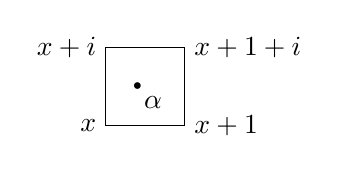
\begin{tikzpicture}
\draw node at (.4,.5) {\tiny$\bullet$};
\node (a) at (.6,.3) {$\alpha$};
\draw (0,0) node[left]{$x$}--(1,0)node[right]{$x+1$}--(1,1)node[right]{$x+1+i$}-- (0,1)node[left]{$x+i$}--cycle; 
\end{tikzpicture} 
 \end{center}
 hat also von einer der $4$ Ecken einen Abstand $\leq \frac{1}{2}\sqrt{2}$. Also existiert ein $x\in\IZ[i]$ mit $\N(x-\alpha)\leq \left( \frac{1}{2}\sqrt{2}\right)^2=\frac{1}{2}<1 $. 
\end{Beweis}

\begin{Folgerung}[EUKLIDischer Algorithmus für $\IZ\lbrack i\rbrack$]
 $\forall m\in\IZ[i], q\in\IZ[i]\oN \exists r,x\in\IZ[i]$ mit:
 \begin{enumerate}
  \item $m=xq+r$
  \item $\N(r)<\N(q)$
 \end{enumerate}

\end{Folgerung}



